% ============================================================
% Reporte: Calculadora de propina con lógica difusa (Mamdani)
% Figuras: capturas de la calculadora web (Playwright) y figuras de
% configuración generadas al ejecutar matlab/propina.fis en GNU Octave
% (reporte/octave/verificar_octave.m).
% Sube a Overleaf este archivo y la carpeta figuras/ (incluye ahí
% tu logo como figuras/IBERO-IE.png). Si agregas capturas de MATLAB
% (figuras/matlab_designer.png, matlab_reglas.png, matlab_ruleview.png),
% aparecen automáticamente en la sección de configuración.
% ============================================================
\documentclass[11pt,letterpaper]{article}

\usepackage[T1]{fontenc}
\usepackage[utf8]{inputenc}
\usepackage[spanish,es-tabla,es-nodecimaldot,es-noshorthands]{babel}
\usepackage{lmodern}
\usepackage[margin=2.5cm,headheight=14pt]{geometry}
\usepackage{amsmath,amssymb}
\usepackage{graphicx}
\usepackage{float}
\usepackage{booktabs}
\usepackage[table]{xcolor}
\usepackage{caption}
\usepackage{subcaption}
\usepackage{enumitem}
\usepackage{fancyhdr}
\usepackage{titlesec}
\usepackage{algorithm}
\usepackage{algpseudocode}
\usepackage{listings}
\usepackage[most]{tcolorbox}
\usepackage[hidelinks]{hyperref}

\definecolor{ibero}{HTML}{D52B1E}
\definecolor{oro}{HTML}{B8860B}
\definecolor{azul}{HTML}{2A78D6}
\definecolor{codigo}{HTML}{F6F6F4}

\titleformat{\section}{\Large\bfseries\color{ibero}}{\thesection}{0.6em}{}
\titleformat{\subsection}{\large\bfseries\color{ibero}}{\thesubsection}{0.6em}{}
\titleformat{\subsubsection}{\normalsize\bfseries}{\thesubsubsection}{0.6em}{}
\captionsetup{font=small,labelfont={bf,color=ibero}}

% --- Datos de la portada (edítalos aquí) ---
\newcommand{\materia}{Lógica Difusa}
\newcommand{\practica}{Práctica: Sistema de Inferencia Difusa}
\newcommand{\alumno}{Carlos Ortega}

\pagestyle{fancy}
\fancyhf{}
\fancyhead[L]{\small \materia}
\fancyhead[R]{\small Propina con lógica difusa Mamdani}
\fancyfoot[C]{\small\thepage}
\renewcommand{\headrule}{{\color{ibero}\hrule height 0.6pt}}

\floatname{algorithm}{Algoritmo}
\renewcommand{\algorithmicrequire}{\textbf{Entrada:}}
\renewcommand{\algorithmicensure}{\textbf{Salida:}}

\lstset{
  basicstyle=\ttfamily\footnotesize,
  backgroundcolor=\color{codigo},
  frame=single, rulecolor=\color{black!15},
  keywordstyle=\color{azul}\bfseries,
  commentstyle=\color{black!55}\itshape,
  stringstyle=\color{ibero},
  breaklines=true, columns=fullflexible,
  xleftmargin=4pt, xrightmargin=4pt, aboveskip=8pt, belowskip=8pt,
}
\lstdefinelanguage{fis}{morecomment=[l]{\%}, morestring=[b]', moredelim=[s][\color{azul}\bfseries]{[}{]}}
\renewcommand{\lstlistingname}{Código}

\newtcolorbox{nota}[1][]{colback=ibero!5,colframe=ibero,boxrule=0.6pt,arc=2pt,left=6pt,right=6pt,top=4pt,bottom=4pt,#1}

\newcommand{\app}{\url{https://sebastiux.github.io/fuzzylogicrestaurante/}}
\newcommand{\repo}{\url{https://github.com/sebastiux/fuzzylogicrestaurante}}
\newcommand{\mf}[1]{\textit{#1}}

\begin{document}

% ------------------------------------------------------------ Portada
\begin{titlepage}
\centering
\IfFileExists{figuras/IBERO-IE.png}{
\includegraphics[width=0.75\textwidth]{figuras/IBERO-IE.png}}{\fbox{\parbox[c][2.5cm][c]{0.42\textwidth}{\centering Logo Ibero\\ \footnotesize(figuras/IBERO-IE.png)}}}\par
\vspace{1.2cm}
{\Large\bfseries Universidad Iberoamericana}\par
\vspace{0.2cm}
{\large \materia}\par
\vspace{1.6cm}
{\color{ibero}\rule{\linewidth}{1.2pt}}\par
\vspace{0.5cm}
{\Huge\bfseries Calculadora de propina}\par
\vspace{0.4cm}
{\LARGE Sistema de inferencia difusa Mamdani:\\[2pt] tiempo de servicio y precio}\par
\vspace{0.4cm}
{\color{ibero}\rule{\linewidth}{1.2pt}}\par
\vspace{0.8cm}
{\large \practica}\par
\vfill
\begin{tabular}{rl}
\textbf{Alumno:} & \textit{\alumno} \\
\textbf{Profesores:} & Dr. Alexandro López González \\
 & Mtro. Julio Caballero Mora \\
\textbf{Fecha:} & \today \\
\end{tabular}\par
\vspace{1cm}
{\small Calculadora: \app\\ Código: \repo}
\end{titlepage}

\tableofcontents
\newpage

% ------------------------------------------------------------
\section{Introducción}

Decidir cuánta propina dejar es un problema de razonamiento aproximado: nadie califica el servicio con un número exacto, sino con expresiones como \emph{``tardaron bastante''} o \emph{``la cuenta salió cara''}. La lógica difusa permite trabajar con este tipo de conceptos vagos, asignando a cada valor numérico un \emph{grado de pertenencia} entre 0 y 1 a conjuntos lingüísticos, y combinarlos con reglas del tipo \emph{si--entonces} para obtener una salida numérica.

En esta práctica se diseña un \textbf{sistema de inferencia difusa tipo Mamdani} con dos entradas, el \textbf{tiempo de servicio} y el \textbf{precio de la cuenta}, y una salida, el \textbf{porcentaje de propina recomendado}. El sistema se define con el \emph{Fuzzy Logic Designer} de MATLAB y se exporta al archivo \texttt{propina.fis}. Ese mismo archivo es leído por una calculadora web publicada en GitHub Pages, que replica la inferencia de \texttt{evalfis} y muestra paso a paso cómo se obtiene la recomendación.

\begin{nota}
\textbf{Calculadora en línea:} \app\qquad \textbf{Código fuente:} \repo
\end{nota}

% ------------------------------------------------------------
\section{Objetivos}

\textbf{General.} Diseñar e implementar un sistema de inferencia difusa Mamdani que recomiende el porcentaje de propina a partir de la relación entre el tiempo de servicio y el precio de la cuenta.

\textbf{Específicos.}
\begin{enumerate}[leftmargin=*]
  \item Definir las variables lingüísticas, sus universos de discurso y sus funciones de pertenencia en el Fuzzy Logic Designer de MATLAB.
  \item Construir una base de reglas que refleje la relación precio--tiempo: una cuenta cara justifica una espera mayor que una barata.
  \item Obtener los datos del sistema con \texttt{evalfis}: grados de pertenencia, fuerza de disparo de las reglas, conjunto agregado y salida defuzzificada.
  \item Publicar una calculadora web que use el mismo archivo \texttt{.fis} y verificar que sus resultados coinciden con una ejecución independiente del sistema.
\end{enumerate}

% ------------------------------------------------------------
\section{Marco teórico}

\subsection{Conjuntos difusos}
Un conjunto difuso $A$ sobre un universo $X$ se define por su función de pertenencia $\mu_A : X \to [0,1]$, que indica en qué grado cada $x$ pertenece a $A$ \cite{zadeh}. A diferencia de un conjunto clásico, un mismo valor puede pertenecer parcialmente a varios conjuntos; por ejemplo, 15 minutos de servicio son a la vez \emph{rápido} en grado $0.5$ y \emph{normal} en grado $0.33$.

\subsection{Funciones de pertenencia}
En este sistema se usan las funciones triangular y trapezoidal, con la misma definición que el Fuzzy Logic Toolbox \cite{mathworks}:
\begin{align}
\text{trimf}(x;a,b,c) &= \max\!\left(\min\!\left(\frac{x-a}{b-a},\ \frac{c-x}{c-b}\right),\ 0\right), \\
\text{trapmf}(x;a,b,c,d) &= \max\!\left(\min\!\left(\frac{x-a}{b-a},\ 1,\ \frac{d-x}{d-c}\right),\ 0\right).
\end{align}
Cuando $a = b$ (o $c = d$) el trapecio tiene un hombro: vale 1 desde el inicio (o hasta el final) del universo.

\subsection{Operadores difusos}
La conjunción (AND) se modela con el mínimo y la disyunción (OR) con el máximo:
\begin{equation}
\mu_{A \wedge B}(x) = \min\big(\mu_A(x),\ \mu_B(x)\big), \qquad \mu_{A \vee B}(x) = \max\big(\mu_A(x),\ \mu_B(x)\big).
\end{equation}

\subsection{Inferencia Mamdani}
En un sistema Mamdani \cite{mamdani} cada regla tiene la forma \emph{si $x_1$ es $A_i$ y $x_2$ es $B_i$ entonces $y$ es $C_i$}, con un conjunto difuso en el consecuente. La inferencia tiene cuatro etapas \cite{ross}:
\begin{enumerate}[leftmargin=*]
  \item \textbf{Fuzzificación.} Se evalúa el grado de pertenencia de cada entrada a sus conjuntos: $\mu_{A_i}(x_1)$, $\mu_{B_i}(x_2)$.
  \item \textbf{Fuerza de disparo.} Se combinan los antecedentes con el operador AND: $w_i = \min\big(\mu_{A_i}(x_1), \mu_{B_i}(x_2)\big)$.
  \item \textbf{Implicación y agregación.} Cada consecuente se recorta a la altura $w_i$ y los conjuntos recortados se unen con el máximo:
  \begin{equation}
  \mu_{\text{agr}}(y) = \max_i \ \min\big(w_i,\ \mu_{C_i}(y)\big).
  \end{equation}
  \item \textbf{Defuzzificación.} El conjunto agregado se convierte en un número con el centroide. MATLAB discretiza el universo de salida en $N = 101$ puntos $y_k$ y calcula
  \begin{equation}
  \label{eq:centroide}
  y^* = \frac{\sum_{k=1}^{N} y_k\, \mu_{\text{agr}}(y_k)}{\sum_{k=1}^{N} \mu_{\text{agr}}(y_k)}.
  \end{equation}
\end{enumerate}

% ------------------------------------------------------------
\section{Planteamiento del problema}

\subsection{Relación entre precio y tiempo}
La idea que guía el diseño es que la tolerancia a la espera depende de lo que se está pagando. En una cuenta cara es razonable que los platillos tarden más, porque suelen ser más elaborados; en una cuenta barata, esperar mucho es una mala experiencia. Por eso un mismo tiempo \emph{lento} se castiga menos cuando el precio es alto, y un servicio \emph{rápido} en una cuenta cara merece la propina más alta.

\subsection{Definición del sistema}

\begin{table}[H]
\centering
\small
\caption{Parámetros generales del sistema de inferencia difusa.}
\label{tab:sistema}
\begin{tabular}{ll}
\toprule
Propiedad & Valor \\
\midrule
Nombre & \texttt{propina} \\
Tipo & Mamdani \\
Entradas & \texttt{tiempo} (min) en $[0, 60]$ y \texttt{precio} (MXN) en $[0, 2000]$ \\
Salida & \texttt{propina} (\%) en $[0, 25]$ \\
AND / OR & \texttt{min} / \texttt{max} \\
Implicación / Agregación & \texttt{min} / \texttt{max} \\
Defuzzificación & \texttt{centroid} (101 puntos) \\
Reglas & 9, todas con conector AND y peso 1 \\
\bottomrule
\end{tabular}
\end{table}

\begin{table}[H]
\centering
\small
\caption{Funciones de pertenencia de las tres variables.}
\label{tab:mfs}
\begin{tabular}{lllll}
\toprule
Variable & Rango & Conjunto & Tipo & Parámetros \\
\midrule
\texttt{tiempo} (min) & $[0, 60]$ & \mf{rapido} & trapmf & $[0\ 0\ 10\ 20]$ \\
 & & \mf{normal} & trimf & $[10\ 25\ 40]$ \\
 & & \mf{lento} & trapmf & $[30\ 45\ 60\ 60]$ \\
\midrule
\texttt{precio} (MXN) & $[0, 2000]$ & \mf{barato} & trapmf & $[0\ 0\ 200\ 600]$ \\
 & & \mf{moderado} & trimf & $[300\ 800\ 1300]$ \\
 & & \mf{caro} & trapmf & $[1000\ 1500\ 2000\ 2000]$ \\
\midrule
\texttt{propina} (\%) & $[0, 25]$ & \mf{muy\_baja} & trapmf & $[0\ 0\ 3\ 6]$ \\
 & & \mf{baja} & trimf & $[3\ 7\ 11]$ \\
 & & \mf{media} & trimf & $[9\ 12.5\ 16]$ \\
 & & \mf{alta} & trimf & $[14\ 18\ 22]$ \\
 & & \mf{muy\_alta} & trapmf & $[20\ 23\ 25\ 25]$ \\
\bottomrule
\end{tabular}
\end{table}

Los conjuntos de cada entrada se traslapan, de modo que cualquier valor del universo activa al menos un conjunto y ninguna combinación de entradas deja al sistema sin reglas activas.

\subsection{Base de reglas}

\begin{table}[H]
\centering
\small
\caption{Base de reglas en forma de matriz: cada celda es el consecuente de la regla \emph{si tiempo es (fila) y precio es (columna)}.}
\label{tab:matriz}
\begin{tabular}{l|ccc}
\toprule
tiempo $\backslash$ precio & \mf{barato} & \mf{moderado} & \mf{caro} \\
\midrule
\mf{rapido} & \mf{alta} (R1) & \mf{alta} (R2) & \mf{muy\_alta} (R3) \\
\mf{normal} & \mf{media} (R4) & \mf{media} (R5) & \mf{alta} (R6) \\
\mf{lento} & \mf{muy\_baja} (R7) & \mf{baja} (R8) & \mf{media} (R9) \\
\bottomrule
\end{tabular}
\end{table}

En cada columna la propina baja conforme el servicio es más lento, y en cada fila sube (o se mantiene) conforme el precio es mayor; ésta es la relación precio--tiempo descrita arriba.

% ------------------------------------------------------------
\section{Configuración en MATLAB}

\subsection{Fuzzy Logic Designer paso a paso}
\begin{enumerate}[leftmargin=*]
  \item Abrir la aplicación con \texttt{fuzzyLogicDesigner} (en R2022b o anteriores, \texttt{fuzzy}) y crear un sistema \textbf{Mamdani} con 2 entradas y 1 salida.
  \item Renombrar las variables a \texttt{tiempo}, \texttt{precio} y \texttt{propina}, y capturar el \emph{Range} de cada una (tabla~\ref{tab:mfs}).
  \item Para cada variable, editar o agregar sus funciones de pertenencia con el nombre, tipo y parámetros de la tabla~\ref{tab:mfs}. La salida necesita cinco funciones.
  \item Fijar los métodos del sistema: And \texttt{min}, Or \texttt{max}, Implication \texttt{min}, Aggregation \texttt{max}, Defuzzification \texttt{centroid}.
  \item Capturar las nueve reglas de la tabla~\ref{tab:matriz} con conector \emph{and} y peso 1.
  \item Verificar en el visor de reglas con la entrada $[15\ 800]$: la propina debe ser $15.89\,\text{\%}$.
  \item Exportar con \emph{Export} $\to$ \emph{To File} como \texttt{propina.fis}.
\end{enumerate}
El repositorio incluye \texttt{matlab/abrir\_designer.m}, que abre el diseñador con todo configurado, y la guía \texttt{matlab/GUIA\_DESIGNER.md} con cada campo a llenar.

\IfFileExists{figuras/matlab_designer.png}{
\begin{figure}[H]
\centering
\includegraphics[width=0.9\textwidth]{figuras/matlab_designer.png}
\caption{Sistema \texttt{propina} en el Fuzzy Logic Designer de MATLAB.}
\end{figure}}{}
\IfFileExists{figuras/matlab_reglas.png}{
\begin{figure}[H]
\centering
\includegraphics[width=0.9\textwidth]{figuras/matlab_reglas.png}
\caption{Editor de reglas de MATLAB con las nueve reglas.}
\end{figure}}{}
\IfFileExists{figuras/matlab_ruleview.png}{
\begin{figure}[H]
\centering
\includegraphics[width=0.9\textwidth]{figuras/matlab_ruleview.png}
\caption{Visor de reglas de MATLAB para tiempo = 15 min y precio = \$800.}
\end{figure}}{}

\subsection{Definición por código}
El mismo sistema se puede construir con la API del Fuzzy Logic Toolbox (R2018b o posterior). El código~\ref{lst:crear} resume \texttt{matlab/crear\_fis\_propina.m}.

\begin{lstlisting}[language=Matlab,caption={Construcción del FIS Mamdani por código.},label={lst:crear}]
fis = mamfis('Name','propina','AndMethod','min','OrMethod','max', ...
    'ImplicationMethod','min','AggregationMethod','max', ...
    'DefuzzificationMethod','centroid');

fis = addInput(fis,[0 60],'Name','tiempo');
fis = addMF(fis,'tiempo','trapmf',[0 0 10 20],'Name','rapido');
fis = addMF(fis,'tiempo','trimf',[10 25 40],'Name','normal');
fis = addMF(fis,'tiempo','trapmf',[30 45 60 60],'Name','lento');

fis = addInput(fis,[0 2000],'Name','precio');
fis = addMF(fis,'precio','trapmf',[0 0 200 600],'Name','barato');
fis = addMF(fis,'precio','trimf',[300 800 1300],'Name','moderado');
fis = addMF(fis,'precio','trapmf',[1000 1500 2000 2000],'Name','caro');

fis = addOutput(fis,[0 25],'Name','propina');
fis = addMF(fis,'propina','trapmf',[0 0 3 6],'Name','muy_baja');
fis = addMF(fis,'propina','trimf',[3 7 11],'Name','baja');
fis = addMF(fis,'propina','trimf',[9 12.5 16],'Name','media');
fis = addMF(fis,'propina','trimf',[14 18 22],'Name','alta');
fis = addMF(fis,'propina','trapmf',[20 23 25 25],'Name','muy_alta');

% [tiempo precio propina peso conector(1 = AND)]
reglas = [1 1 4 1 1; 1 2 4 1 1; 1 3 5 1 1;
          2 1 3 1 1; 2 2 3 1 1; 2 3 4 1 1;
          3 1 1 1 1; 3 2 2 1 1; 3 3 3 1 1];
fis = addRule(fis, reglas);
writeFIS(fis,'propina');
\end{lstlisting}

\subsection{Archivo \texttt{propina.fis}}
El código~\ref{lst:fis} muestra las secciones principales del archivo exportado; es el que lee la calculadora web.

\begin{lstlisting}[language=fis,caption={Extracto de \texttt{matlab/propina.fis}.},label={lst:fis}]
[System]
Name='propina'
Type='mamdani'
NumInputs=2
NumOutputs=1
NumRules=9
AndMethod='min'
OrMethod='max'
ImpMethod='min'
AggMethod='max'
DefuzzMethod='centroid'

[Input1]
Name='tiempo'
Range=[0 60]
NumMFs=3
MF1='rapido':'trapmf',[0 0 10 20]
MF2='normal':'trimf',[10 25 40]
MF3='lento':'trapmf',[30 45 60 60]

[Rules]
1 1, 4 (1) : 1
1 2, 4 (1) : 1
1 3, 5 (1) : 1
...
3 3, 3 (1) : 1
\end{lstlisting}

\subsection{Funciones de pertenencia}
Las figuras~\ref{fig:mf-entradas} y~\ref{fig:mf-salida} se obtuvieron ejecutando \texttt{plotmf} sobre \texttt{propina.fis} en GNU Octave 8.4 con el paquete \texttt{fuzzy-logic-toolkit} \cite{octave}, compatible con la sintaxis de MATLAB (script \path{reporte/octave/verificar_octave.m}).

\begin{figure}[H]
\centering
\begin{subfigure}{0.49\textwidth}
\centering
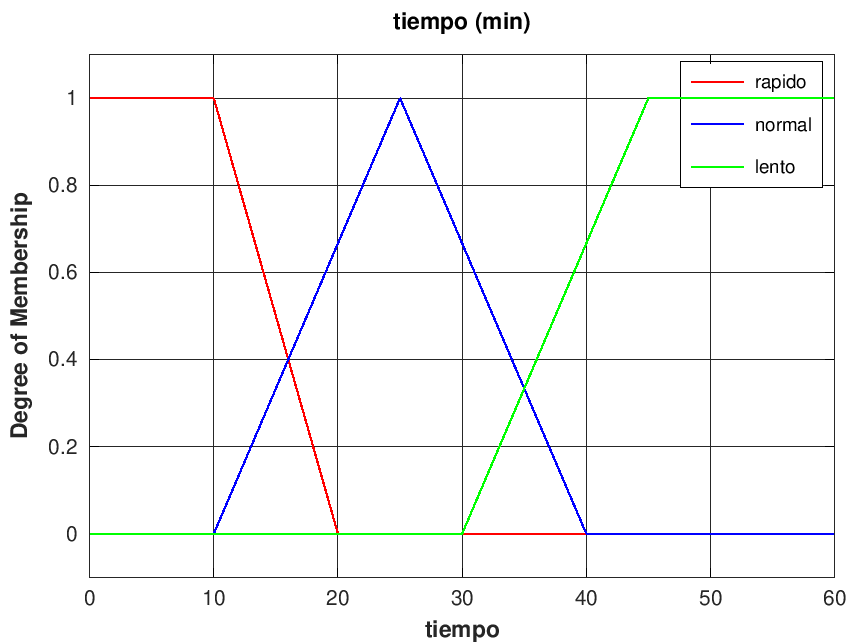
\includegraphics[width=\textwidth]{figuras/oct_mf_tiempo.png}
\caption{Tiempo de servicio.}
\end{subfigure}\hfill
\begin{subfigure}{0.49\textwidth}
\centering
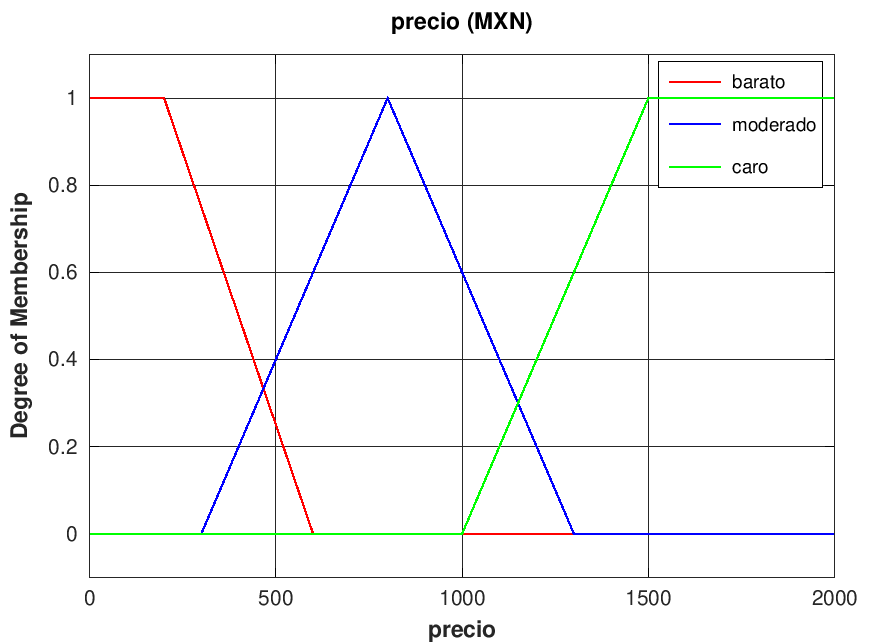
\includegraphics[width=\textwidth]{figuras/oct_mf_precio.png}
\caption{Precio de la cuenta.}
\end{subfigure}
\caption{Funciones de pertenencia de las entradas (\texttt{plotmf}).}
\label{fig:mf-entradas}
\end{figure}

\begin{figure}[H]
\centering
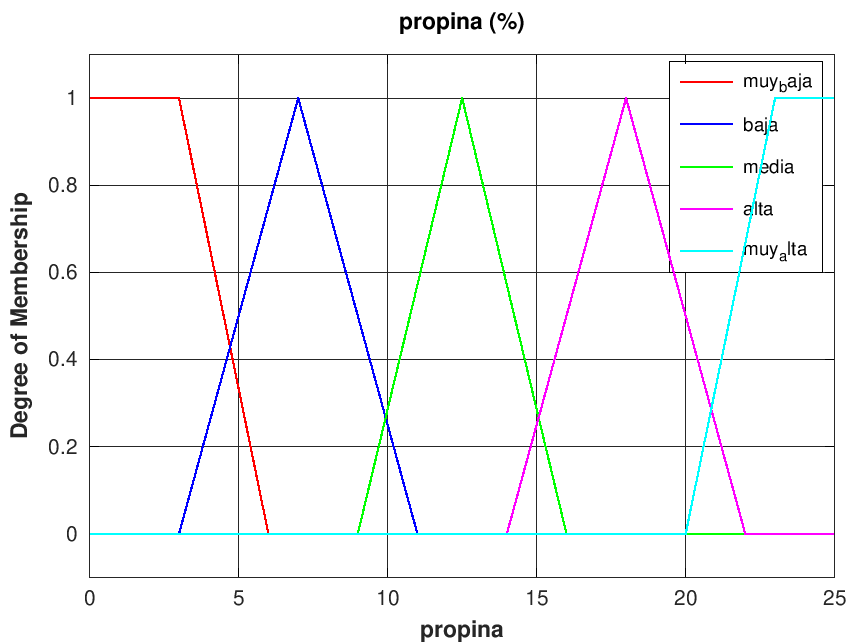
\includegraphics[width=0.6\textwidth]{figuras/oct_mf_propina.png}
\caption{Funciones de pertenencia de la salida \texttt{propina} (\texttt{plotmf}).}
\label{fig:mf-salida}
\end{figure}

% ------------------------------------------------------------
\section{Calculadora web}

\subsection{Arquitectura}
La calculadora es una página estática (HTML, CSS y JavaScript con módulos ES, sin dependencias externas) publicada en GitHub Pages:
\begin{itemize}[leftmargin=*]
  \item \textbf{Motor difuso} (\texttt{js/fuzzy.js}): lee el archivo \texttt{.fis} de MATLAB y replica \texttt{evalfis} para sistemas Mamdani: las mismas definiciones de \texttt{trimf}, \texttt{trapmf} y otras funciones, los operadores \texttt{min}/\texttt{max}/\texttt{prod}/\texttt{probor}, la agregación y la defuzzificación sobre 101 puntos.
  \item \textbf{Interfaz} (\texttt{js/app.js}): controles de entrada, resultado, gráficas de fuzzificación y del conjunto agregado, tabla de reglas con su fuerza de disparo y superficie de control.
\end{itemize}
El diseño, la programación y la verificación del sistema se hicieron con apoyo del asistente de inteligencia artificial Claude \cite{claude}. Como la página carga \texttt{matlab/propina.fis} al iniciar, cualquier cambio exportado desde el Fuzzy Logic Designer y subido al repositorio se refleja en la calculadora sin modificar el código.

\begin{algorithm}[H]
\caption{Inferencia Mamdani implementada en la calculadora}
\label{alg:mamdani}
\begin{algorithmic}[1]
\Require FIS leído de \texttt{propina.fis}, entradas $(x_1, x_2)$
\Ensure Porcentaje de propina $y^*$
\State Saturar cada $x_j$ a su rango
\For{cada regla $i$}
  \State $w_i \gets \min\big(\mu_{A_i}(x_1),\ \mu_{B_i}(x_2)\big)$ \Comment{fuerza de disparo}
\EndFor
\State $y_k \gets$ 101 puntos equiespaciados en $[0, 25]$
\For{cada $y_k$}
  \State $\mu_{\text{agr}}(y_k) \gets \max_i \min\big(w_i,\ \mu_{C_i}(y_k)\big)$ \Comment{implicación y agregación}
\EndFor
\State $y^* \gets \sum_k y_k\,\mu_{\text{agr}}(y_k) \big/ \sum_k \mu_{\text{agr}}(y_k)$ \Comment{centroide}
\State \Return $y^*$
\end{algorithmic}
\end{algorithm}

\subsection{Interfaz}

\begin{figure}[H]
\centering
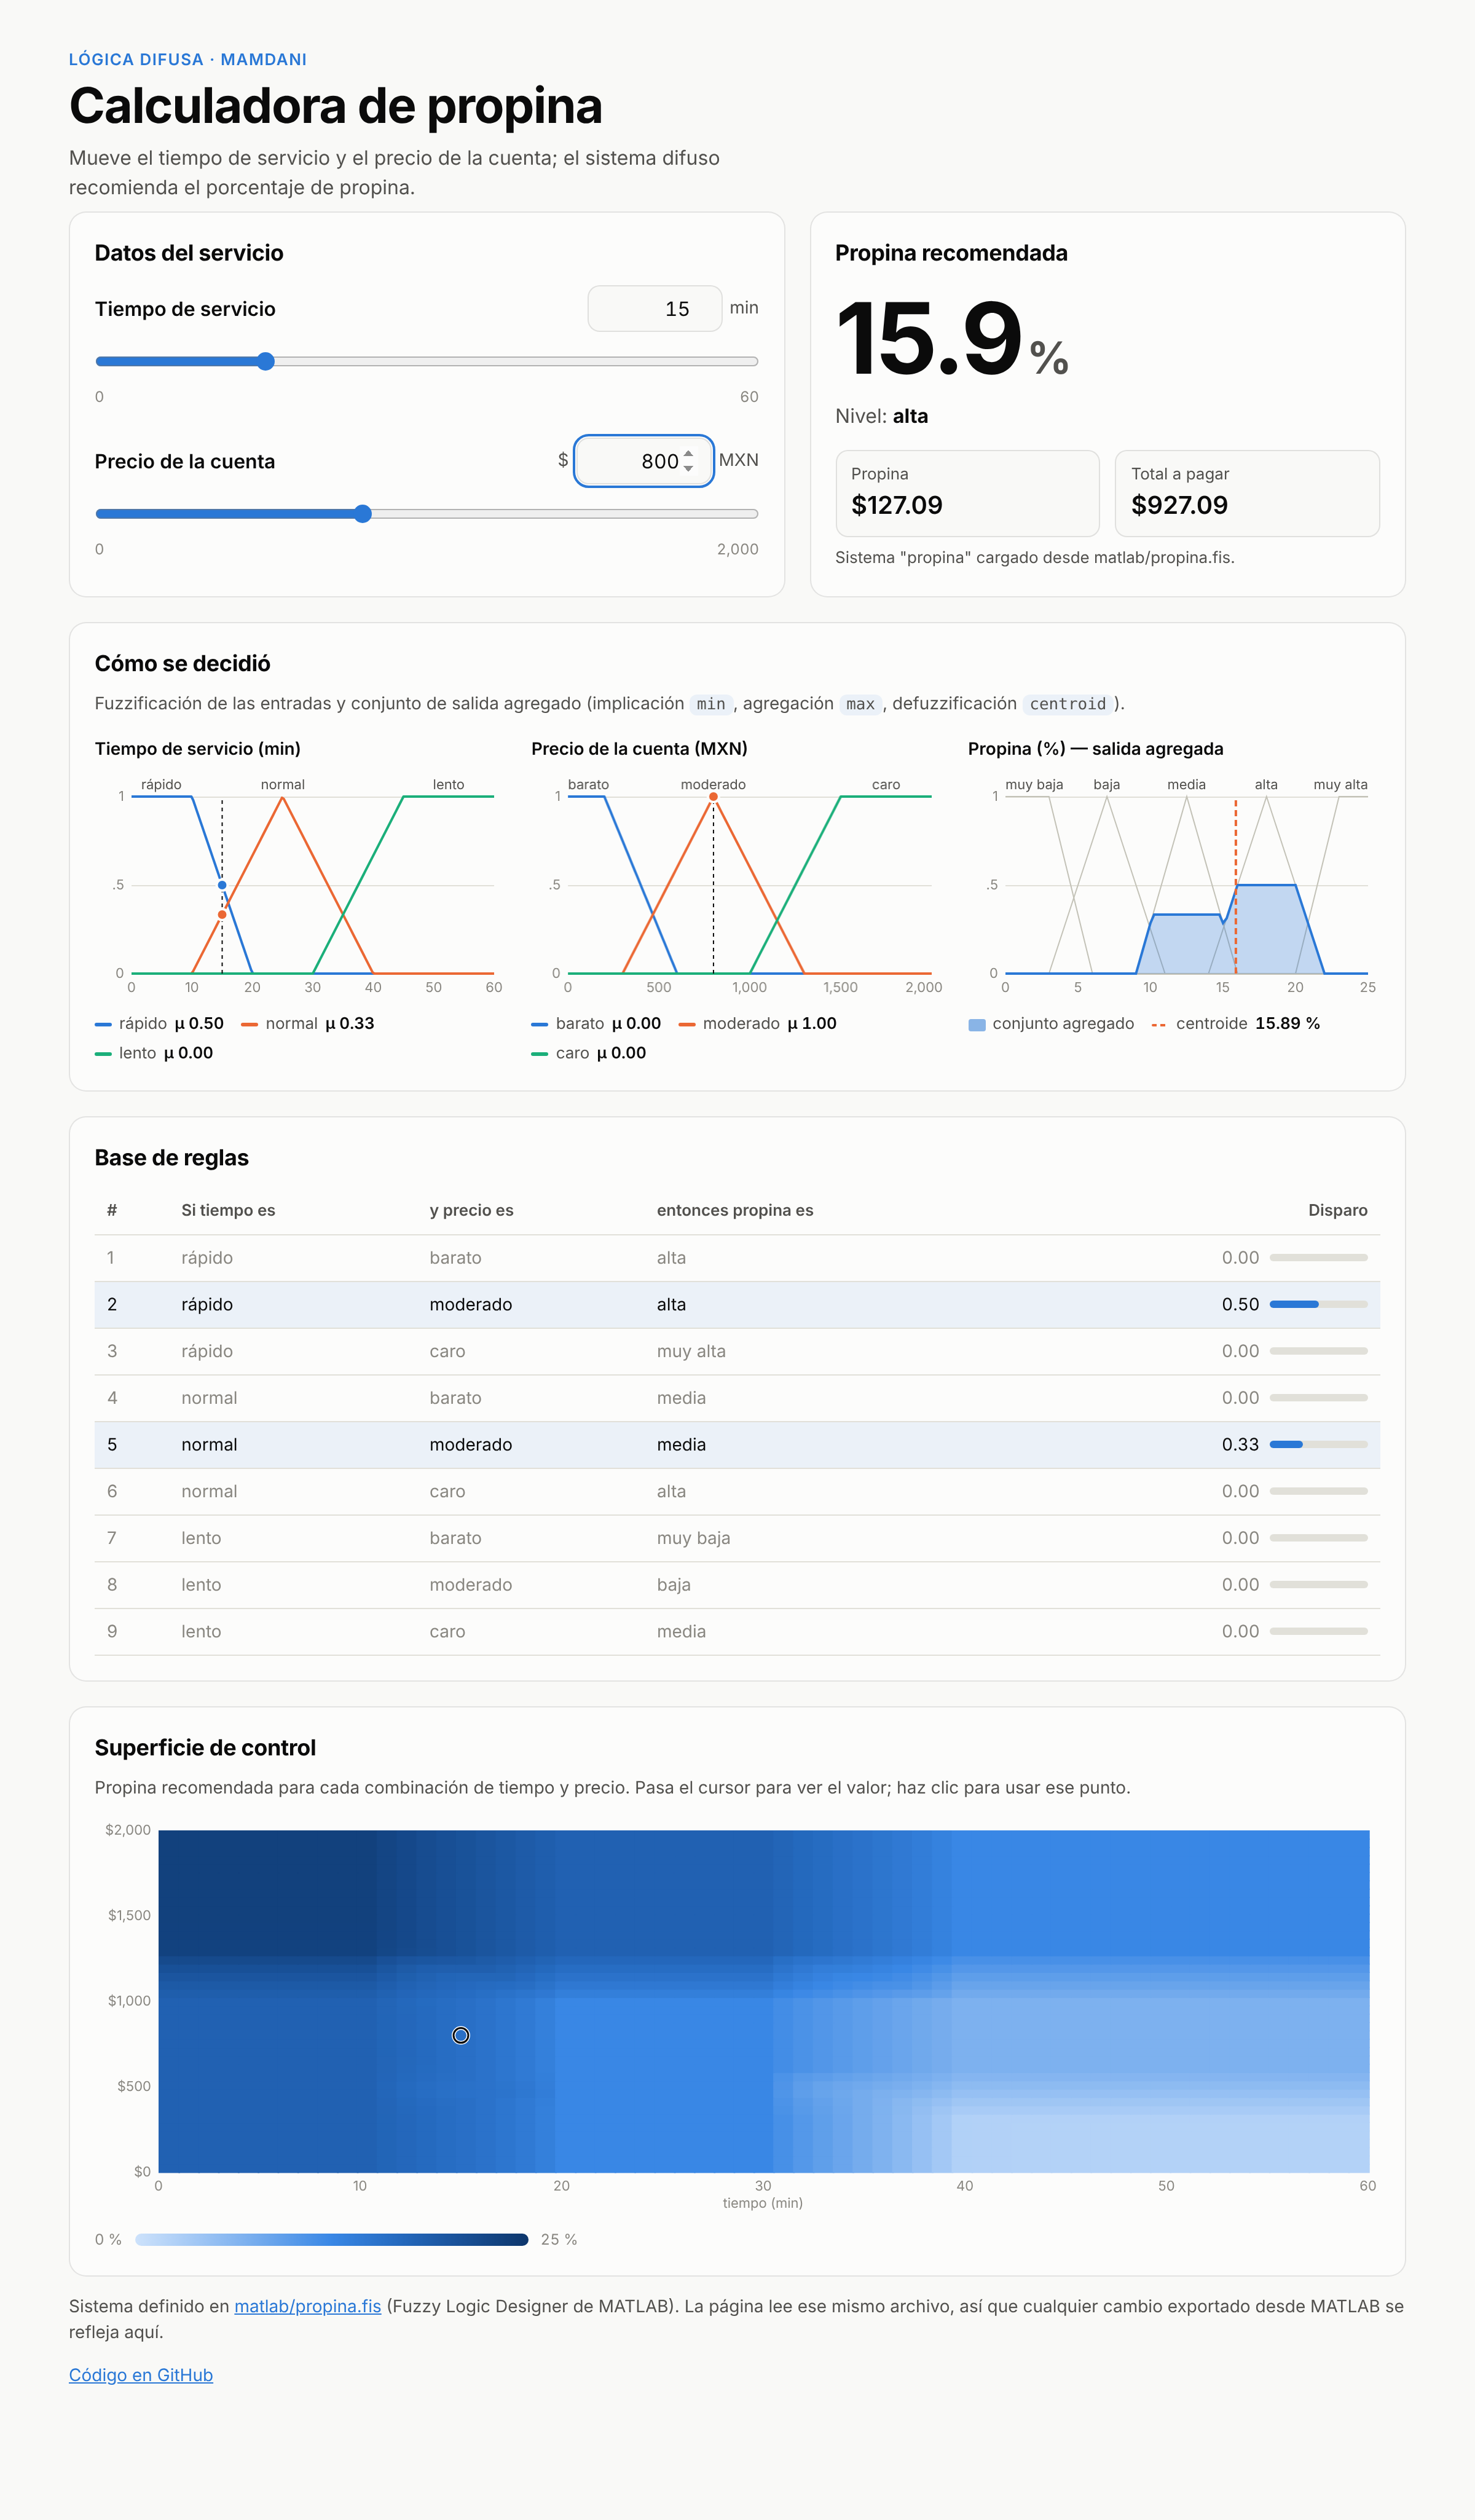
\includegraphics[height=0.78\textheight,keepaspectratio]{figuras/fig_app_completa.png}
\caption{Vista completa de la calculadora con tiempo = 15 min y precio = \$800.}
\label{fig:app}
\end{figure}

\begin{figure}[H]
\centering
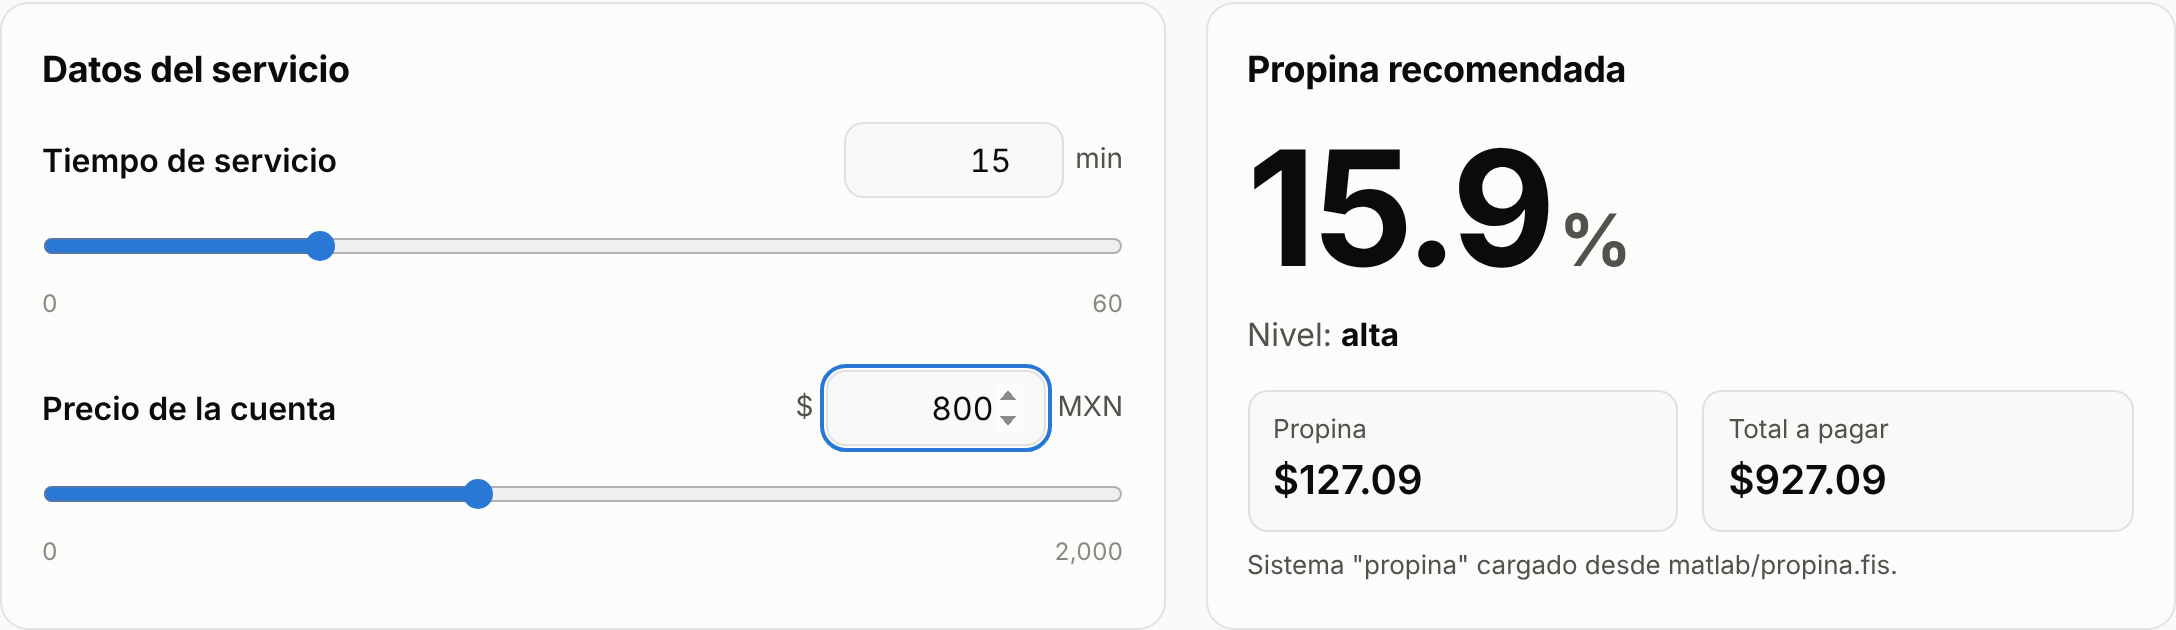
\includegraphics[width=\textwidth]{figuras/fig_app_resultado.png}
\caption{Entradas y resultado: propina recomendada, nivel lingüístico, monto de la propina y total a pagar.}
\label{fig:app-resultado}
\end{figure}

\begin{figure}[H]
\centering
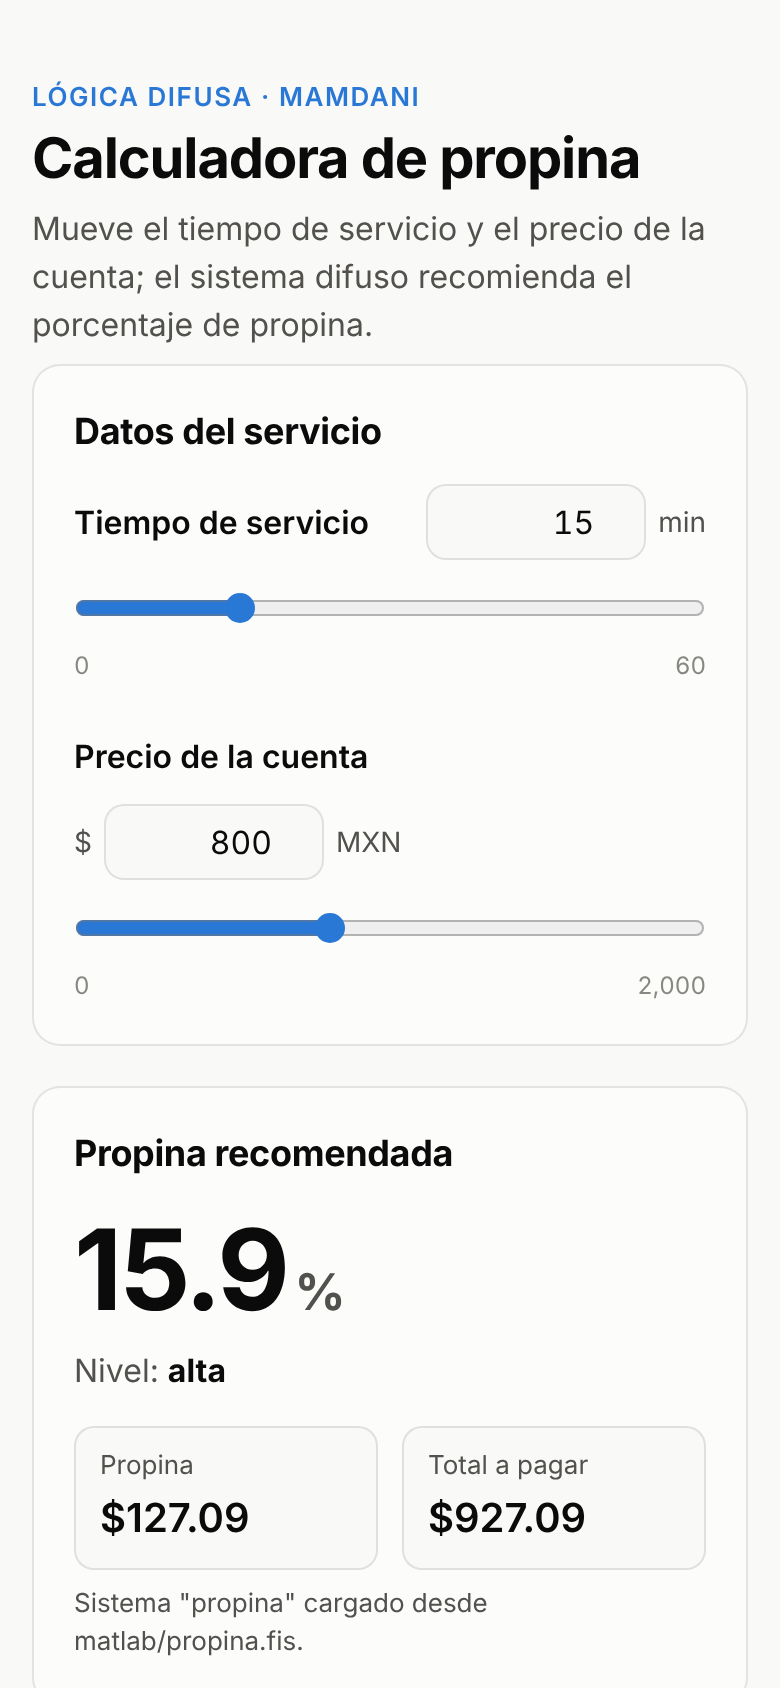
\includegraphics[width=0.3\textwidth]{figuras/fig_app_movil.png}
\caption{La calculadora en un teléfono.}
\label{fig:app-movil}
\end{figure}

% ------------------------------------------------------------
\clearpage
\section{Resultados paso a paso}

\subsection{Caso 1: tiempo = 15 min, precio = \$800}

\paragraph{Paso 1: fuzzificación.} Con las funciones de la tabla~\ref{tab:mfs}:
\begin{align*}
\mu_{\text{rapido}}(15) &= \frac{20 - 15}{20 - 10} = 0.50, &
\mu_{\text{normal}}(15) &= \frac{15 - 10}{25 - 10} = 0.33, &
\mu_{\text{lento}}(15) &= 0, \\
\mu_{\text{barato}}(800) &= 0, &
\mu_{\text{moderado}}(800) &= 1, &
\mu_{\text{caro}}(800) &= 0.
\end{align*}
Quince minutos son ``algo rápido y algo normal'', y \$800 es plenamente ``moderado''.

\paragraph{Paso 2: fuerza de disparo.} Cada regla toma el mínimo de sus antecedentes. Sólo se activan las reglas que combinan \mf{rapido} o \mf{normal} con \mf{moderado}:

\begin{table}[H]
\centering
\small
\caption{Fuerza de disparo de las nueve reglas para la entrada $[15\ 800]$.}
\label{tab:disparo}
\begin{tabular}{clllccc}
\toprule
Regla & tiempo & precio & propina & $\mu(\text{tiempo})$ & $\mu(\text{precio})$ & $w_i = \min$ \\
\midrule
R1 & \mf{rapido} & \mf{barato} & \mf{alta} & $0.50$ & $0$ & $0$ \\
\rowcolor{azul!10} R2 & \mf{rapido} & \mf{moderado} & \mf{alta} & $0.50$ & $1$ & $\mathbf{0.50}$ \\
R3 & \mf{rapido} & \mf{caro} & \mf{muy\_alta} & $0.50$ & $0$ & $0$ \\
R4 & \mf{normal} & \mf{barato} & \mf{media} & $0.33$ & $0$ & $0$ \\
\rowcolor{azul!10} R5 & \mf{normal} & \mf{moderado} & \mf{media} & $0.33$ & $1$ & $\mathbf{0.33}$ \\
R6 & \mf{normal} & \mf{caro} & \mf{alta} & $0.33$ & $0$ & $0$ \\
R7 & \mf{lento} & \mf{barato} & \mf{muy\_baja} & $0$ & $0$ & $0$ \\
R8 & \mf{lento} & \mf{moderado} & \mf{baja} & $0$ & $1$ & $0$ \\
R9 & \mf{lento} & \mf{caro} & \mf{media} & $0$ & $0$ & $0$ \\
\bottomrule
\end{tabular}
\end{table}

\paragraph{Paso 3: implicación y agregación.} El conjunto \mf{alta} se recorta a $0.50$ y \mf{media} a $0.33$; su unión con el máximo da el conjunto agregado:
\begin{equation*}
\mu_{\text{agr}}(y) = \max\Big(\min\big(0.50,\ \mu_{\text{alta}}(y)\big),\ \min\big(0.33,\ \mu_{\text{media}}(y)\big)\Big).
\end{equation*}

\begin{table}[H]
\centering
\small
\caption{Valores del conjunto agregado en algunos puntos del universo de salida.}
\label{tab:agregado}
\begin{tabular}{l*{10}{c}}
\toprule
$y$ (\%) & 9 & 10 & 11 & 12.5 & 14 & 15 & 15.5 & 16 & 20 & 22 \\
\midrule
$\mu_{\text{agr}}(y)$ & $0$ & $0.286$ & $0.333$ & $0.333$ & $0.333$ & $0.286$ & $0.375$ & $0.500$ & $0.500$ & $0$ \\
\bottomrule
\end{tabular}
\end{table}

\paragraph{Paso 4: defuzzificación.} Con los 101 puntos $y_k = 0, 0.25, \ldots, 25$ y la ecuación~\eqref{eq:centroide}:
\begin{equation*}
y^* = \frac{\sum_k y_k\,\mu_{\text{agr}}(y_k)}{\sum_k \mu_{\text{agr}}(y_k)} = \frac{297.1979}{18.7083} = \mathbf{15.89\,\text{\%}}.
\end{equation*}
El resultado queda entre \mf{media} y \mf{alta}, más cerca de \mf{alta} porque esa regla dispara con más fuerza. Para una cuenta de \$800 la propina es de \$127.09 y el total, \$927.09 (figura~\ref{fig:app-resultado}).

\begin{figure}[H]
\centering
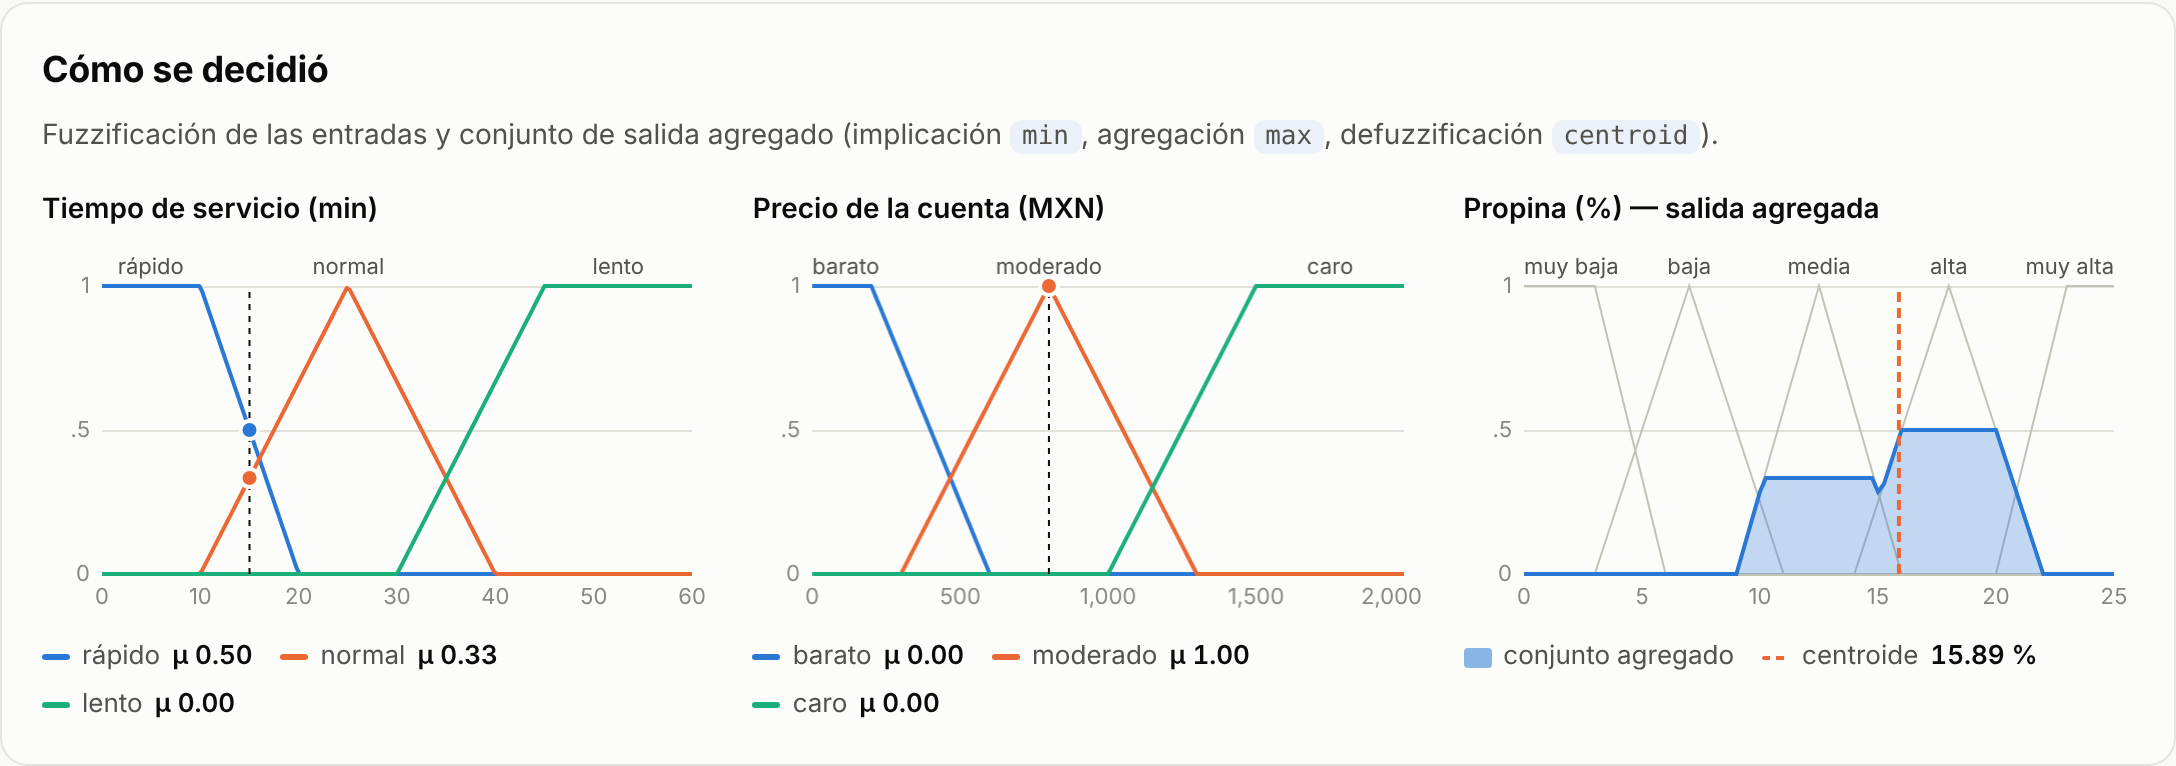
\includegraphics[width=\textwidth]{figuras/fig_app_inferencia.png}
\caption{Fuzzificación y conjunto agregado en la calculadora para $[15\ 800]$. La línea punteada naranja es el centroide.}
\label{fig:app-inferencia}
\end{figure}

\begin{figure}[H]
\centering
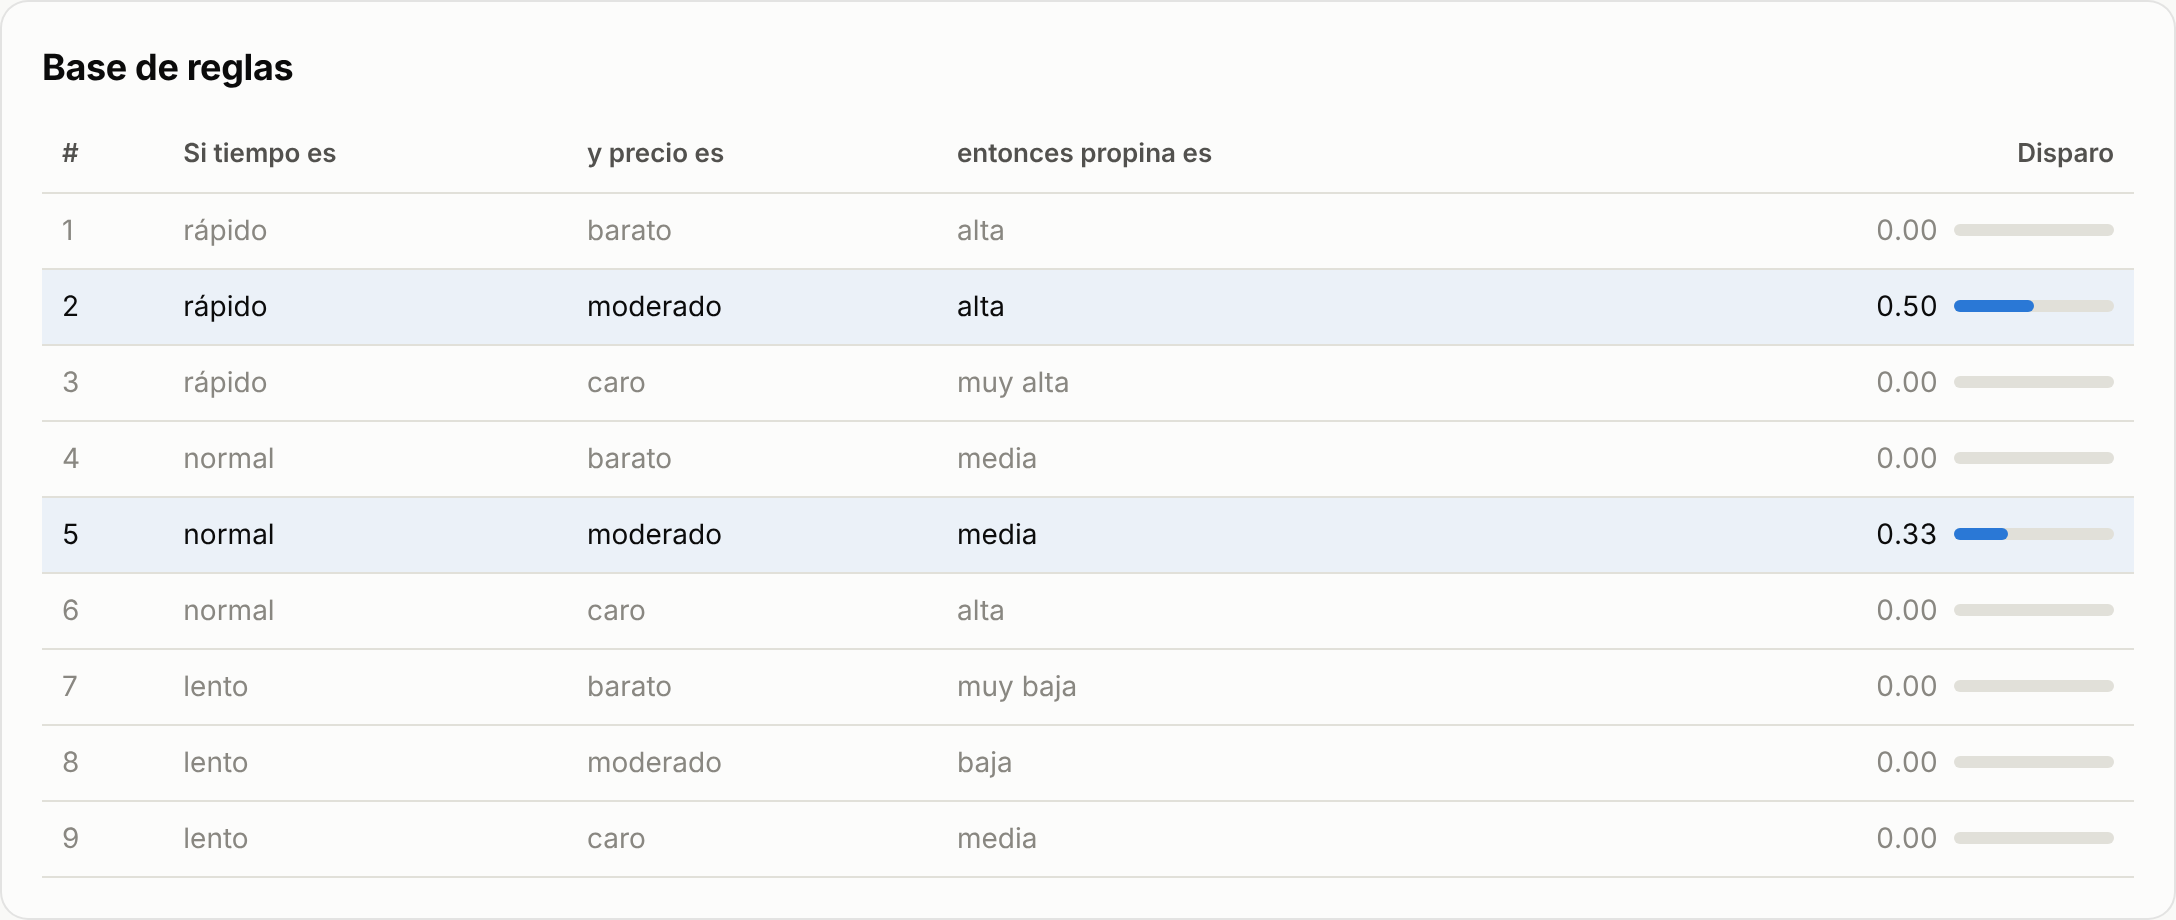
\includegraphics[width=\textwidth]{figuras/fig_app_reglas.png}
\caption{Base de reglas en la calculadora: se resaltan R2 ($w = 0.50$) y R5 ($w = 0.33$).}
\label{fig:app-reglas}
\end{figure}

\begin{figure}[H]
\centering
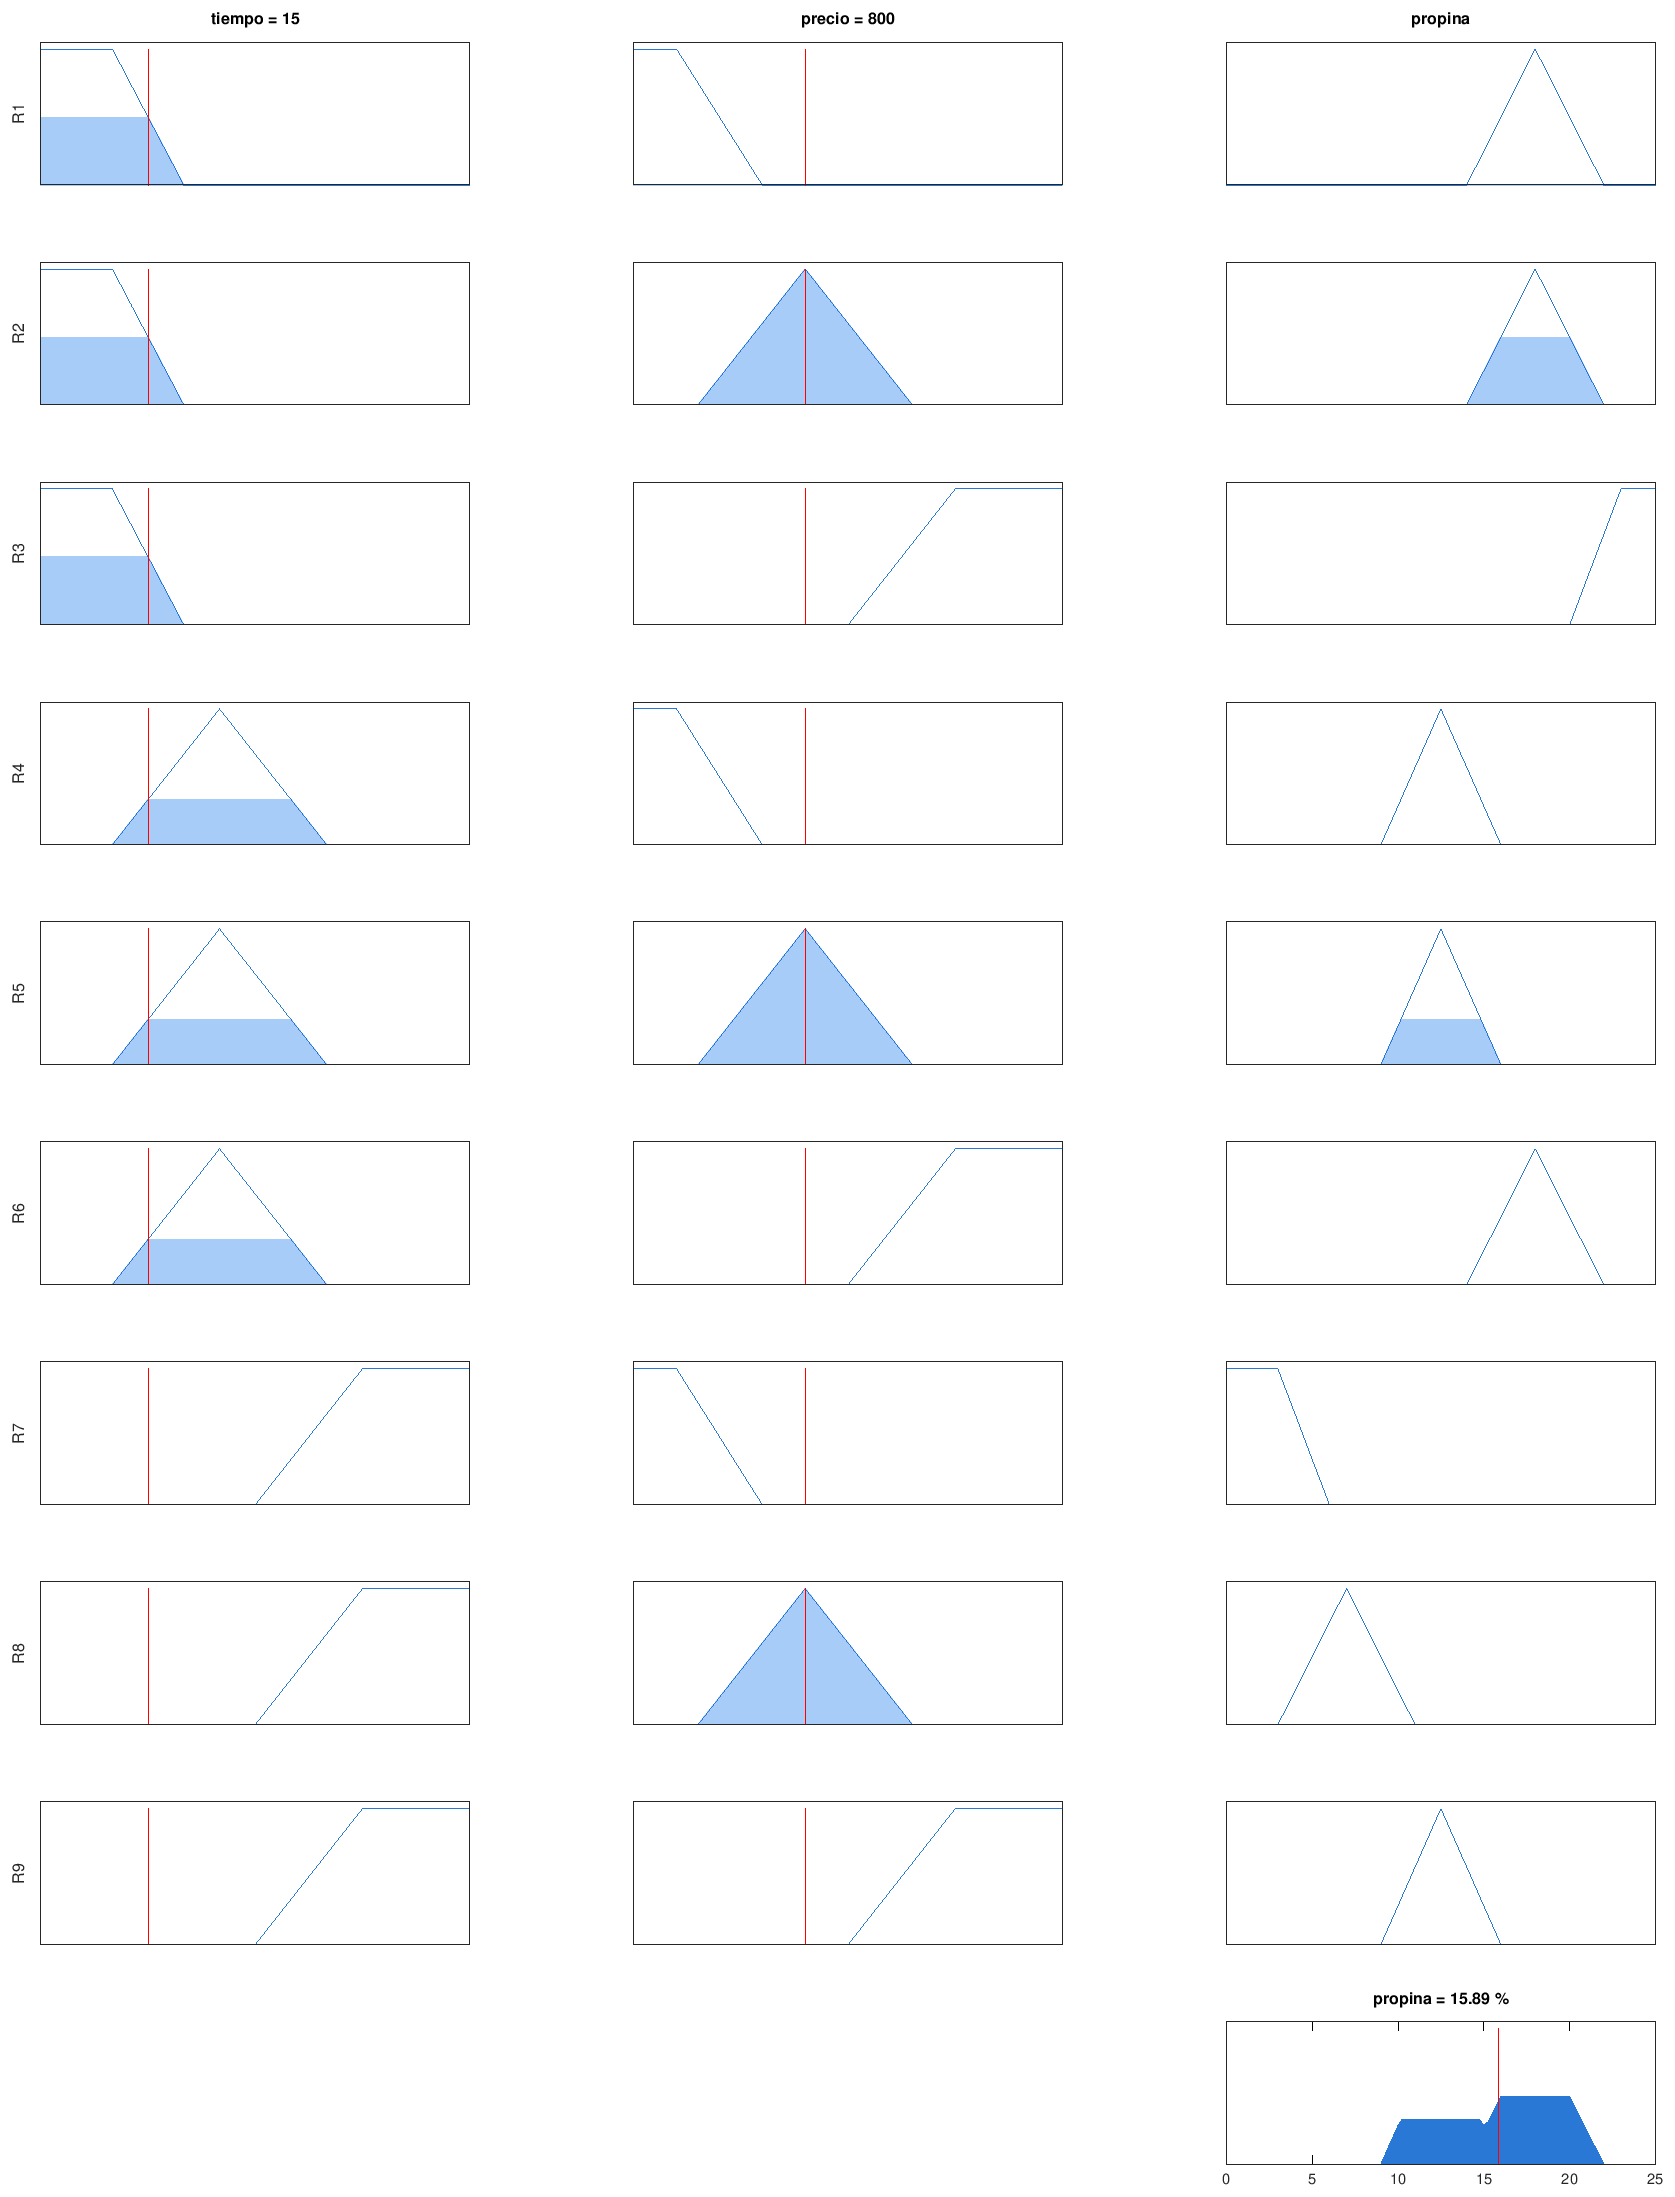
\includegraphics[height=0.62\textheight,keepaspectratio]{figuras/oct_ruleview.png}
\caption{Visor de reglas para $[15\ 800]$ generado en Octave con las salidas de \texttt{evalfis}: en cada fila, los antecedentes (área sombreada hasta el grado de pertenencia) y el consecuente recortado; abajo, el conjunto agregado y el centroide.}
\label{fig:ruleview}
\end{figure}

\subsection{Caso 2: tiempo = 42 min, precio = \$1{,}500}
Ahora el servicio es lento, $\mu_{\text{lento}}(42) = \frac{42-30}{45-30} = 0.80$, y la cuenta es cara, $\mu_{\text{caro}}(1500) = 1$. Sólo dispara R9 (\emph{lento y caro $\Rightarrow$ media}) con $w_9 = 0.80$. El conjunto agregado es \mf{media} recortado a $0.80$, simétrico alrededor de $12.5$, así que
\begin{equation*}
y^* = \frac{167.8571}{13.4286} = \mathbf{12.50\,\text{\%}}.
\end{equation*}
Este caso muestra la relación precio--tiempo: con la misma lentitud y una cuenta barata la regla activa sería R7 y la propina caería a $2.27\,\text{\%}$.

\begin{figure}[H]
\centering
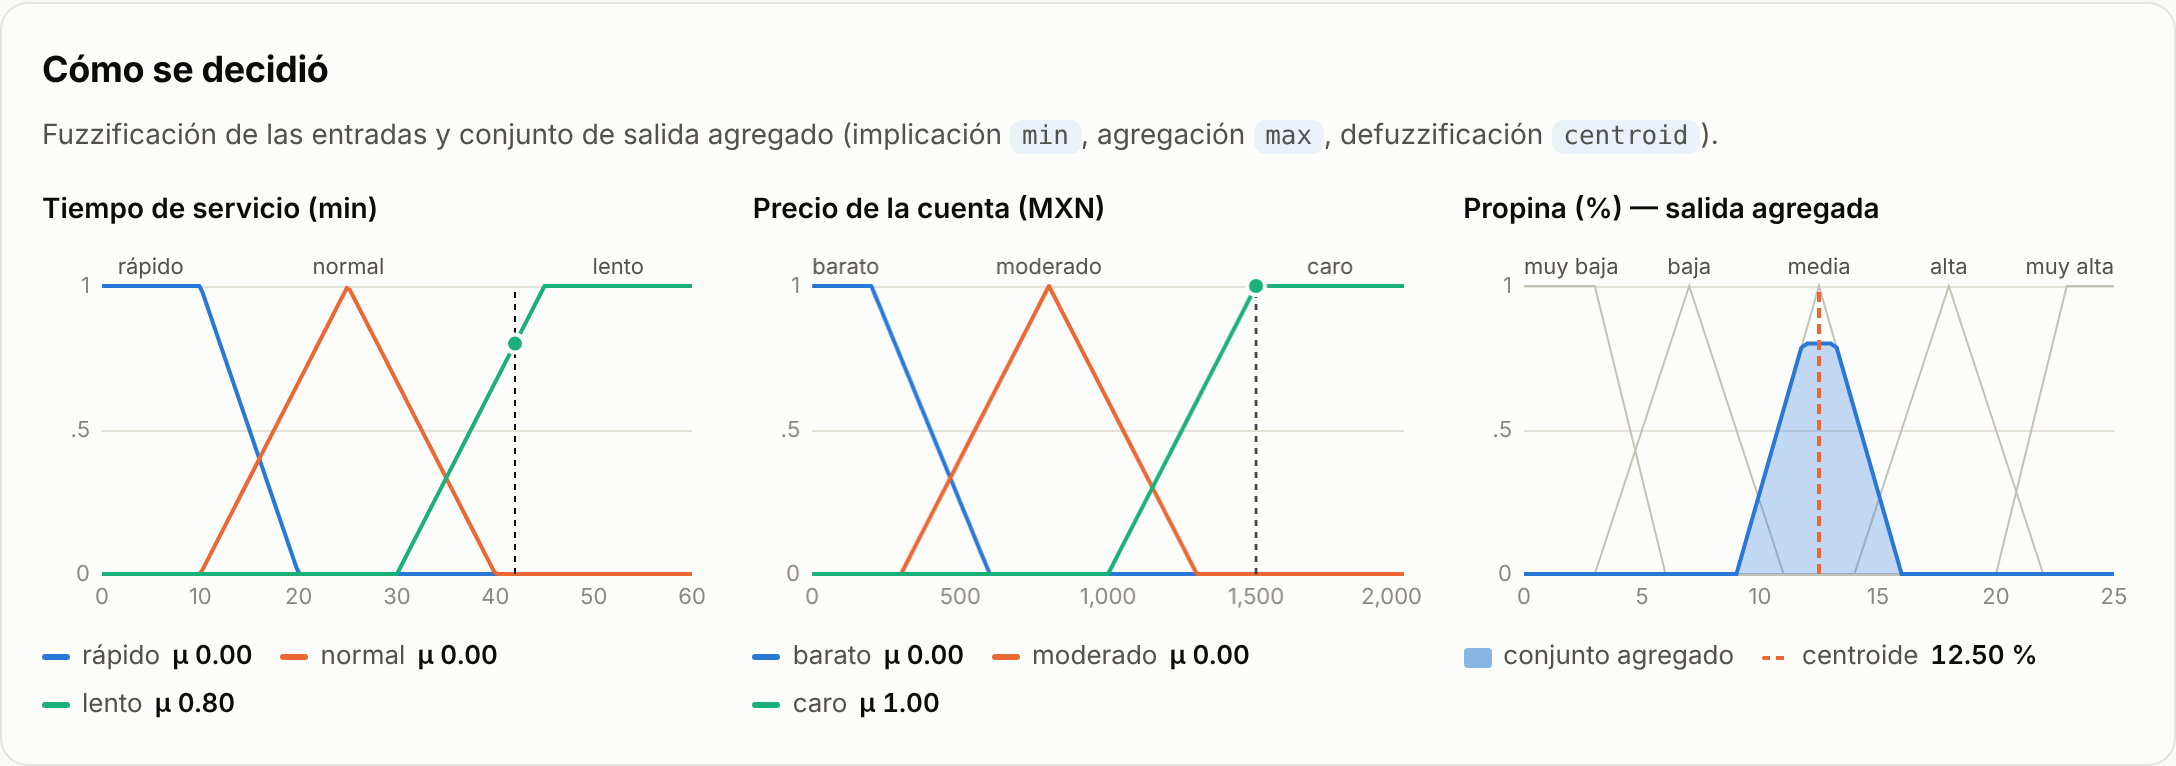
\includegraphics[width=\textwidth]{figuras/fig_app_caso2_inferencia.png}
\caption{Caso 2 en la calculadora: sólo dispara la regla R9.}
\label{fig:caso2}
\end{figure}

% ------------------------------------------------------------
\section{Superficie de control y casos de prueba}

\begin{figure}[H]
\centering
\begin{subfigure}{0.49\textwidth}
\centering
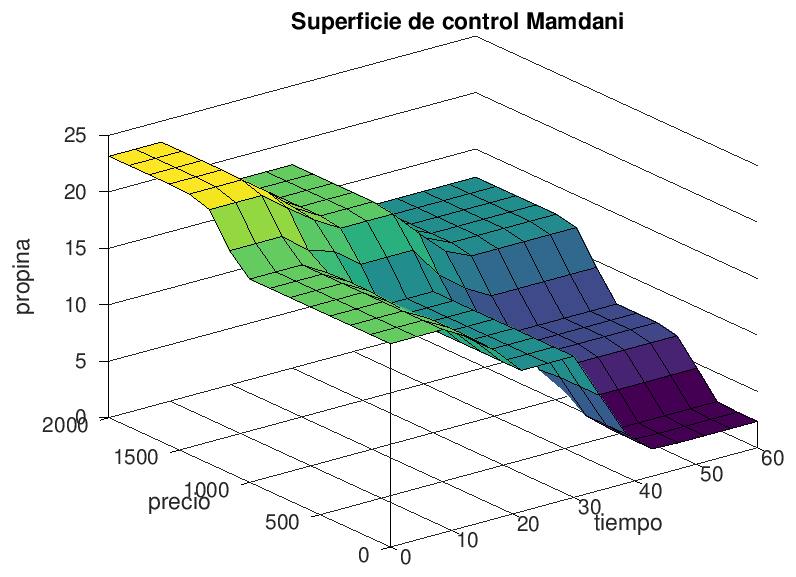
\includegraphics[width=\textwidth]{figuras/oct_superficie.png}
\caption{\texttt{gensurf} en Octave.}
\end{subfigure}\hfill
\begin{subfigure}{0.49\textwidth}
\centering
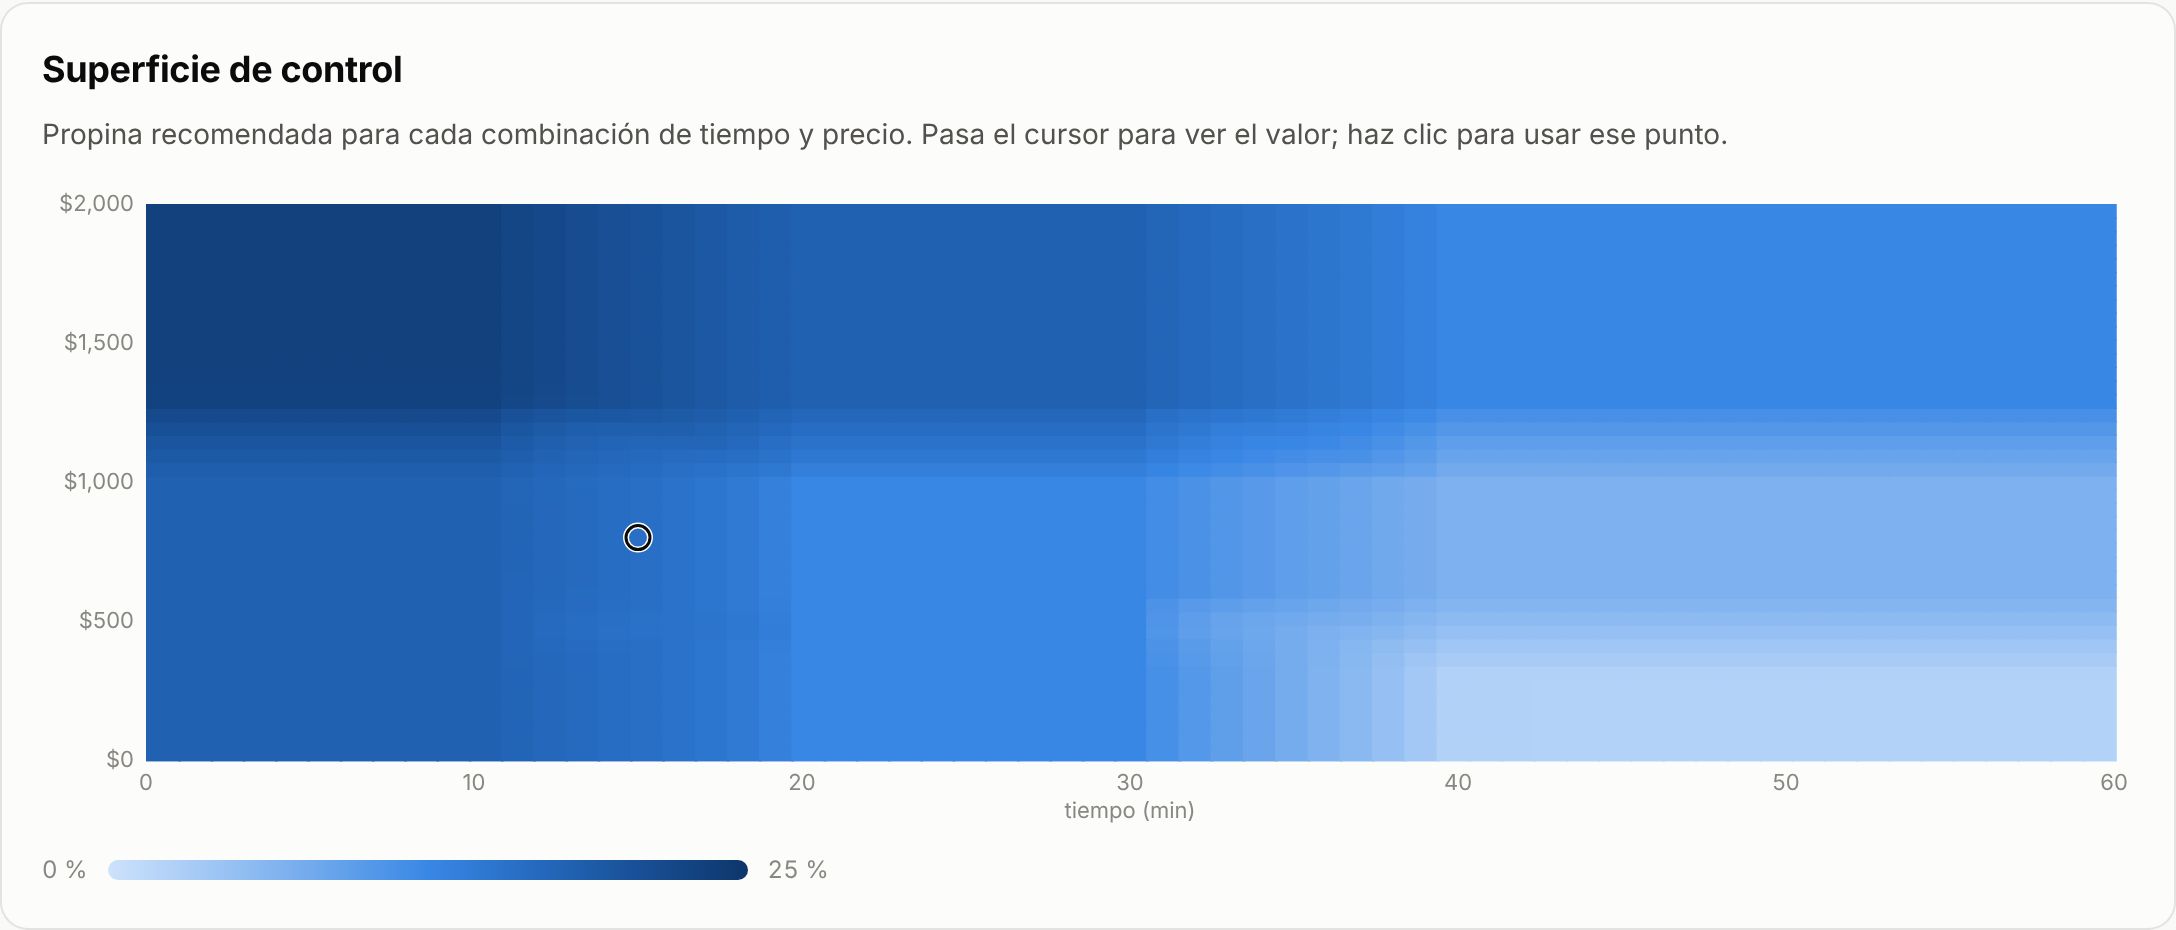
\includegraphics[width=\textwidth]{figuras/fig_app_superficie.png}
\caption{Mapa de calor en la calculadora.}
\end{subfigure}
\caption{Superficie de control: propina recomendada para cada combinación de tiempo y precio.}
\label{fig:superficie}
\end{figure}

La superficie confirma el diseño: la propina disminuye conforme aumenta el tiempo y, para un mismo tiempo, aumenta con el precio. Las mesetas corresponden a zonas donde una sola regla domina; las rampas, a las transiciones entre conjuntos.

\begin{table}[H]
\centering
\small
\caption{Casos de prueba. La columna \emph{Calculadora} usa el centroide discreto de MATLAB (ecuación~\ref{eq:centroide}); la columna \emph{Octave} es la ejecución independiente de \texttt{propina.fis} con \texttt{evalfis}.}
\label{tab:casos}
\begin{tabular}{rrlrrr}
\toprule
tiempo (min) & precio (MXN) & situación & Calculadora (\%) & Octave (\%) & diferencia \\
\midrule
5 & 150 & rápido, barato & $18.00$ & $18.00$ & $0$ \\
5 & 800 & rápido, moderado & $18.00$ & $18.00$ & $0$ \\
5 & 1800 & rápido, caro & $23.21$ & $23.15$ & $0.06$ \\
25 & 150 & normal, barato & $12.50$ & $12.50$ & $0$ \\
25 & 800 & normal, moderado & $12.50$ & $12.50$ & $0$ \\
25 & 1800 & normal, caro & $18.00$ & $18.00$ & $0$ \\
50 & 150 & lento, barato & $2.27$ & $2.33$ & $-0.06$ \\
50 & 800 & lento, moderado & $7.00$ & $7.00$ & $0$ \\
50 & 1800 & lento, caro & $12.50$ & $12.50$ & $0$ \\
15 & 450 & transición & $15.60$ & $15.60$ & $0$ \\
15 & 800 & caso 1 & $15.89$ & $15.89$ & $0$ \\
35 & 1100 & transición & $11.66$ & $11.66$ & $0$ \\
42 & 1500 & caso 2 & $12.50$ & $12.50$ & $0$ \\
\bottomrule
\end{tabular}
\end{table}

\subsection{Verificación}
Para validar la calculadora se evaluó \texttt{propina.fis} en una malla de $61 \times 41 = 2501$ puntos (tiempo de 0 a 60 cada minuto, precio de 0 a 2000 cada \$50) con dos implementaciones independientes: el motor web y \texttt{evalfis} de Octave.
\begin{itemize}[leftmargin=*]
  \item Las únicas diferencias aparecen cuando el conjunto agregado toca un extremo del universo de salida (0\,\text{\%} o 25\,\text{\%}), con un máximo de $0.09$ puntos porcentuales. Se deben a que Octave calcula el centroide por integración trapezoidal, $\int y\,\mu\,dy \big/ \int \mu\,dy$ con \texttt{trapz}, que da la mitad de peso a los puntos extremos, mientras que MATLAB y la calculadora usan la suma discreta de la ecuación~\eqref{eq:centroide}.
  \item Si el motor web usa también \texttt{trapz}, la diferencia máxima con Octave en los 2501 puntos es de $5 \times 10^{-15}$, es decir, error de redondeo. Por lo tanto, la fuzzificación, la fuerza de disparo, la implicación y la agregación coinciden exactamente.
\end{itemize}

\begin{nota}
El paquete de Octave exige $a < b$ en \texttt{trapmf}, mientras que MATLAB acepta hombros con $a = b$. Para la verificación los hombros se extendieron una unidad fuera del rango (por ejemplo, $[0\ 0\ 10\ 20] \to [-1\ 0\ 10\ 20]$), lo que no cambia ningún valor dentro del universo de discurso.
\end{nota}

% ------------------------------------------------------------
\section{Obtención de datos en MATLAB}
El script \texttt{matlab/exportar\_datos.m} reúne los comandos para extraer todos los datos del sistema Mamdani. Los principales son:

\begin{lstlisting}[language=Matlab,caption={Extracción de datos con \texttt{evalfis}.},label={lst:datos}]
fis  = readfis('propina.fis');
opts = evalfisOptions('NumSamplePoints',101);

% Salida para un caso
p = evalfis(fis,[15 800],opts)                 % 15.8859

% Detalle de la inferencia (ruleFiring requiere R2019b o posterior)
[p,fuzzIn,ruleOut,aggOut,ruleFiring] = evalfis(fis,[15 800],opts);
%   fuzzIn     : grados de pertenencia por regla y entrada (9x2)
%   ruleFiring : fuerza de disparo de cada regla (9x1)
%   aggOut     : conjunto agregado en los 101 puntos

% Superficie completa a CSV
[T,P] = meshgrid(0:1:60, 0:50:2000);
Z = reshape(evalfis(fis,[T(:) P(:)],opts), size(T));
writetable(table(T(:),P(:),Z(:),'VariableNames', ...
    {'tiempo_min','precio_mxn','propina_pct'}),'superficie_propina.csv');

% Graficas
plotmf(fis,'input',1); plotmf(fis,'input',2); plotmf(fis,'output',1);
gensurf(fis); plotfis(fis); ruleview(fis)
\end{lstlisting}

% ------------------------------------------------------------
\section{Conclusiones}
\begin{enumerate}[leftmargin=*]
  \item El sistema Mamdani traduce reglas expresadas en lenguaje natural en una recomendación numérica continua: con 3 conjuntos por entrada, 5 en la salida y 9 reglas se obtiene una superficie de control suave entre $2.27\,\text{\%}$ y $23.21\,\text{\%}$.
  \item La base de reglas captura la relación precio--tiempo: para un servicio lento la propina pasa de $2.27\,\text{\%}$ con una cuenta barata a $12.50\,\text{\%}$ con una cara, porque una cuenta cara tolera más espera.
  \item Las salidas intermedias de \texttt{evalfis} (grados de pertenencia, fuerza de disparo y conjunto agregado) permiten reconstruir a mano cada recomendación, como en el caso de 15 min y \$800, cuyo centroide es $15.89\,\text{\%}$.
  \item La calculadora web lee el mismo archivo \texttt{.fis} que MATLAB y reproduce su inferencia; al compararla con una ejecución independiente en Octave sobre 2501 puntos sólo difiere por el método numérico del centroide en los extremos del universo de salida.
\end{enumerate}

% ------------------------------------------------------------
\begin{thebibliography}{9}
\bibitem{zadeh} L.~A. Zadeh, ``Fuzzy sets,'' \emph{Information and Control}, vol.~8, no.~3, pp.~338--353, 1965.
\bibitem{mamdani} E.~H. Mamdani y S.~Assilian, ``An experiment in linguistic synthesis with a fuzzy logic controller,'' \emph{International Journal of Man-Machine Studies}, vol.~7, no.~1, pp.~1--13, 1975.
\bibitem{ross} T.~J. Ross, \emph{Fuzzy Logic with Engineering Applications}, 4.ª ed. Chichester: Wiley, 2016.
\bibitem{mathworks} The MathWorks, Inc., \emph{Fuzzy Logic Toolbox User's Guide}. Natick, MA. Disponible en \url{https://www.mathworks.com/help/fuzzy/}.
\bibitem{octave} L.~Markowsky, \emph{Fuzzy Logic Toolkit for GNU Octave}, versión 0.4.6. Disponible en \url{https://gnu-octave.github.io/packages/fuzzy-logic-toolkit/}.
\bibitem{claude} Anthropic, \emph{Claude} (asistente de inteligencia artificial, usado mediante Claude Code), 2026. Utilizado como apoyo en el diseño del sistema difuso, la programación de la calculadora web, la verificación en Octave y la redacción de este reporte. Disponible en \url{https://claude.ai}.
\end{thebibliography}

\end{document}
